\documentclass[journal]{IEEEtran}
\usepackage{graphicx}
\usepackage{hyperref}
%\usepackage[spanish, mexico]{babel}
\begin{document}

\title{Modelo para la Detección de Posturas de Yoga Usando Redes Neuronales Convolucionales}

\author{\IEEEauthorblockN{Oskar Ramses Beltran Magaña}\\
\IEEEauthorblockA{\textit{Universidad Veracruzana} \\
\textit{Facultad de Ingeniería Eleéctrica y Electrónica}\\
Veracruz, Mexico \\
oskarr.magana@gmail.com}
}

\maketitle

\begin{abstract}
Yoga is a discipline many people want to get involved to due to its benefits on general well being. The new lifestyles derived in the necessity of systems that are able to teach and supervise the execution of yoga postures. This project proposes model that classifies yoga postures using computer vision and convolutional neural networks. 
\end{abstract}

\begin{IEEEkeywords}
yoga, pose, detection, CNN.
\end{IEEEkeywords}

\section{Introducción}

\IEEEPARstart{E}{ntre} las distintas causas de lesiones al ejercitarse, podemos encontrar la incorrecta ejecución de las actividades \cite{10.1145/3010915.3010941}. Por otro lado, para la recuperación en algunas de estas lesiones es necesario realizar otro grupo de ejercicios cuya efectividad viene dada a partir de la adecuada ejecución de estos \cite{10.1145/2856767.2856773}. Sin embargo, no siempre es posible supervisar que las actividades se realicen apropiadamente, por lo que un sistema que sea capaz de realizar esta tarea permitiría aumentar la eficacia de las rutinas.

La Yoga es una filosofía que, además ideas espirituales y filosofías alimentarias, utiliza distintas posturas muy marcadas que requieren de su correcta ejecución para conseguir diversos efectos en el cuerpo de quien las lleva a cabo. Debido a los efectos que estas posturas pueden tener en el bienestar de quien las hace, es que la gente busca practicarlas sin embargo al no siempre es posible asistir con un maestro yogi que supervise el desarrollo de estos ejercicios.

Por ello, esta investigación tiene como objetivo el desarrollar un modelo que explore la capacidad de identificar entre cinco poses distintas a partir de una clasificación simple.

\section{Estado del Arte}
En la detección de posturas humanas han existido distintas aproximaciones y el caso de la yoga no es la excepción. Los principales enfoques para para detección de estas han sido dos: una sóla persona y múltiples individuos. 
Así pues, en la línea de una sola persona, Palanimeera y Ponmozhi \cite{palanimeera2021classification} crearon un algoritmo de dibuja un esqueleto sobre el individuo y comparan la eficacia de cuatro algoritmos diferentes a la hora de clasificar la postura del saludo al sol, siendo el de K vecinos más cercanos el de mayor eficacia con un 96\% de precisión. Bhosale et al. \cite{bhosale2022yoga} proponen el uso de una librería pre-existente para la detección de las posturas y, posteriormente, a través de un algoritmo de K vecinos más cercanos realizar la clasificación de entre 5 posturas diferentes. Haciendo uso también de los K vecinos más cercanos. Una propuesta interesante es la que se propone en \cite{anand2022yoga} donde el modelo busca no sólo aprender de un set de datos preexistente, si no que toma un video que el usuario agrega para determinar y corregir las posturas de este. Esta propuesta realiza un dibujado de las articulaciones para crear una figura del sujeto y con ella evaluar las posturas a través de cuatro modelos distintos, siendo el de redes convolucionales el que mejor resultado demuestra, siendo sólo superado por las combinaciones de las redes neuronales convolucionales con redes de memoria de corto-largo plazo. \cite{8666736} hace eco de la eficacia de las redes convolucionales y utiliza su implementación en tercera dimensión para analizar posturas a partir de videos, utilizando algoritmos que identifican articulaciones y las preservan a través del tiempo para hacer un seguimiento a través de los movimientos que hacen las personas al tomar estas posturas. 

En el caso de la detección de poses de varios individuos, YogNet \cite{yadav2022yognet}, de forma parecida a Anand et al. combina redes convolucionales con redes de memoria corto-largo plazo dividiendo el flujo de información en dos, enfocando la primera a la detección de características posturales y la segunda en las espacio-temporales. 

\section{Diseño e implementación}

En el diseño de este modelo se trabajó en dos fases, la primera se centró en la investigación y recolección del Set de datos, posteriormente se hizo un ligero preprocesado imágenes en el cual se intentó sacar las características más esenciales de las imágenes para que a partir de esto se diseñara modelo de Red neuronal con evolucionar el cual será capaz de distinguir entre cinco posturas de yoga diferentes. Éste modelo se sometió a un proceso de entrenamiento de aproximadamente 300 épocas.

\subsection{Conjunto de datos}
Para el conjunto de datos se utilizó uno preexistente en la plataforma Kaggle conformada por más de 1500 imágenes distribuidas en cinco posturas de yoga: perro boca abajo (downdog), árbol (tree), tabla (plank), guerrero 2 (warrior2) y diosa (goddess) \cite{pandit_2020}. 

\subsection{Modelo}
La red neuronal se conforma de una capa convolucional de entrada, dos convolucionales y una densa en la capa oculta y otra capa densa en la capa de salida, con cinco salidas correspondientes a las cinco categorías o posturas. Este se puede ver a más detalle en ta Tabla 1.
\begin{table}[h!]
    \centering
    \begin{tabular}{c c c}
    \hline
    \\
    Tipo de capa & Salida & \# Parámetros\\
    \\
    \hline
     conv2D (capa de entrada) & (None, 146, 96, 32) & 832 \\
     MaxPooling2D & (None, 73, 48, 32) & 0 \\
     Conv2D & (None, 69, 44, 64) & 51264 \\  
     MaxPooling2D & (None, 34, 22, 64) & 0 \\
     Conv2D & (None, 30, 18, 128) & 204928 \\  
     MaxPooling2D & (None, 15, 9, 128) & 0 \\
     Flatten & (None, 17280) & 0 \\
     Dense & (None, 1000) & 17281000 \\
     Dense (capa de salida) & (None, 5) & 5005 \\
    \hline
    \\
    Parámetros totales: 17,543,029 \\
    Parámetros entrenables: 17,543,029 \\
    Parámetros no entrenables: 0 \\
    \hline
    \\
    \end{tabular}
    \caption{Arquitectura de la red neuronal.}
    \label{tab:1}
\end{table}

\section{Resultados}

A través del entrenamiento del modelo este demostró una eficacia del 99.65\% sin embargo al contrastar con el conjunto de validación vemos que consigue acertar en un 94.48\%. Como podemos ver en la Fig. 1, lar curvas de entrenamiento y validación empiezan a divergir a partir de 160 épocas. 

\begin{figure}[htbp]
    \centering
    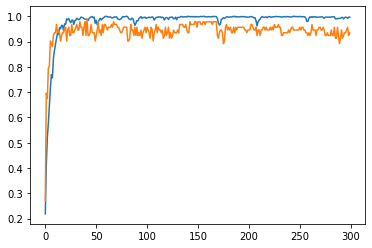
\includegraphics[width=0.8\columnwidth]{5x5-3convlayers300epochs.png}
    \caption{Precisión del modelo, conjunto de entrenamiento (azul) vs conjunto de prueba (naranja).}
    \label{fig:acurracy}
\end{figure}

Por otro lado, al evaluar el error, la función de pérdida nos arroja un valor de 0.0091 que contrasta fuertemente con el 0.4804 que arroja el conjunto de entrenamiento, valor que en ningún momento converge durante el proceso de entrenamiento y validación tal y como se puede ver en la fig. 2. 

\begin{figure}[htbp]
    \centering
    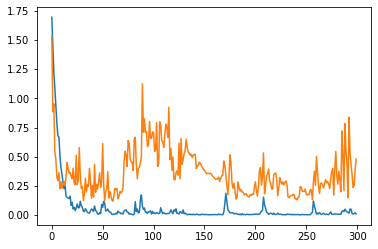
\includegraphics[width=0.8\columnwidth]{loss-5x5-3convlayers300epochs.png}
    \caption{Función de pérdida, conjunto de entrenamiento (azul) vs conjunto de prueba (naranja).}
    \label{fig:loss}
\end{figure}

\section{Conclusión y trabajo futuro}
Como ya se mencionó, después de las 160 épocas el modelo parece caer en un sobre entrenamiento, aún así, con una precisión del 94.48\% el modelo cumple su objetivo al clasificar entre las posturas, sin embargo es necesario seguir trabajando más en el pre-procesado de las imágenes pues con la puntuación de error demuestra que no diferencia con total certeza entre las categorías. Una detección de la posición de cada extremidad, tal y como otros autores han propuesto, podría ayudar a reducir este valor. 

Por otra parte, el set de datos con el que se trabajó contaba con muy pocas muestras en general y pocas categorías. Con el fin de posteriormente desarrollar un sistema de aprendizaje de yoga es necesario un conjunto más robusto que incluya un mayor número de posturas y muestras para cada una de estas, tal y como podría ser el conjunto propuesto por Verma et al. \cite{9151085}. Además, este sistema debe ser capaz de dar retroalimentación al usuario durante la ejecución de la actividad y no una vez se ha realizado dicha pose. 

Por otra parte, no fue posible comprobar de primera mano la detección de posturas puesto que el grupo de investigación no es conocedor de yoga, por lo cual en un futuro trabajo se buscará a un practicante experimentado para poner a prueba el modelo.

\appendices
\section{}
Todo el código relacionado a este trabajo se encuentra en \url{https://github.com/rakso-dev/TIA_proyecto}.

\section{}
El acceso al conjunto de datos se encuentra en \url{https://www.kaggle.com/datasets/niharika41298/yoga-poses-dataset}.
\ifCLASSOPTIONcaptionsoff
  \newpage
\fi

\bibliographystyle{ieeetr}
\bibliography{bibtex/bib/Referencias}

\end{document}


